\documentclass[a4]{scrartcl}

% \usepackage[ngerman]{babel}
\usepackage[utf8]{inputenc}
\usepackage{mathtools}
\usepackage{amsmath}
\usepackage{amssymb}
\usepackage{geometry}
\usepackage{scrlayer-scrpage}
\usepackage{float}
\usepackage{xcolor}
\pagestyle{scrheadings}
\usepackage{stmaryrd}
\let\stmaryrdLightning\lightning
\clearscrheadfoot

\usepackage[backend=biber, maxbibnames=99]{biblatex}
\addbibresource{references.bib}

\setlength{\parindent}{0cm}


\geometry{
  paper=a4paper, % Change to letterpaper for US letter
  top=2cm, % Top margin
  bottom=1.5cm, % Bottom margin
  left=2cm, % Left margin
  right=3cm, % Right margin
}

\ohead{\\
Pina Kolling\\
piko0011}

\usepackage[framemethod=TikZ]{mdframed}

% Style %
\mdfdefinestyle{enviStyle}{
   innertopmargin = 10pt,
  linewidth      = 1pt,
  frametitlerule = true,
  roundcorner    = 2pt%
}


\newenvironment{CountingDefinition}[2][]{%
   \ifstrempty{#1}%
   {\mdfsetup{%
      frametitle={{\strut ~}}}
   }%
   {\mdfsetup{%
      frametitle={{\strut ~#1}}}%
   }%
   \mdfsetup{
      nobreak                   = true,
     linecolor                 = gray,
    frametitlebackgroundcolor = gray!50,
    style                     = enviStyle
   }
   \begin{mdframed}[]\relax%
   \label{#2}}{\end{mdframed}}

\begin{document}

\section*{Summary: Lecture 8}

Summary for the chapters \textit{9.3} and \textit{9.4}. \cite{book, CC}





%---------------------------------------------------------------



\begin{CountingDefinition}[Undirected graph]{def:validLabelPlacement}

An undirected graph $G$ is a pair of sets $(V, E)$ where $V$ is the finite set of nodes and $E$ is a set of unordered pairs in $V$ that are symmetric: 
\begin{align*}
\forall \ i,j \in E, i \neq j: \  (i, j) \in E \Rightarrow (j, i) \in E 
\end{align*}

\end{CountingDefinition}








%---------------------------------------------------------------

\subsection*{\textsc{IndependentSet}}

\begin{CountingDefinition}[\textsc{IndependentSet}]{def:validLabelPlacement}

Input: An undirected Graph $G = (V, E)$ and a number $k$.
\ \\
Question: Is there a set $I \subseteq V$ of $k = |I|$ nodes with no edges in between? (\textsc{IndependentSet})
\end{CountingDefinition}

\begin{CountingDefinition}[\textsc{3SAT}]{def:validLabelPlacement}
Like the \textsc{Sat} problem, \textsc{3Sat} is determining the satisfiability of a formula in CNF where each clause is limited to at most three literals.
\end{CountingDefinition}

\textsc{IndependentSet} is NP-complete.

\ \\
\textbf{Proof idea:}
\begin{itemize}
\item triangle construction: any independent set can contain at most one node of the triangle
\begin{figure}[H]
\begin{center}
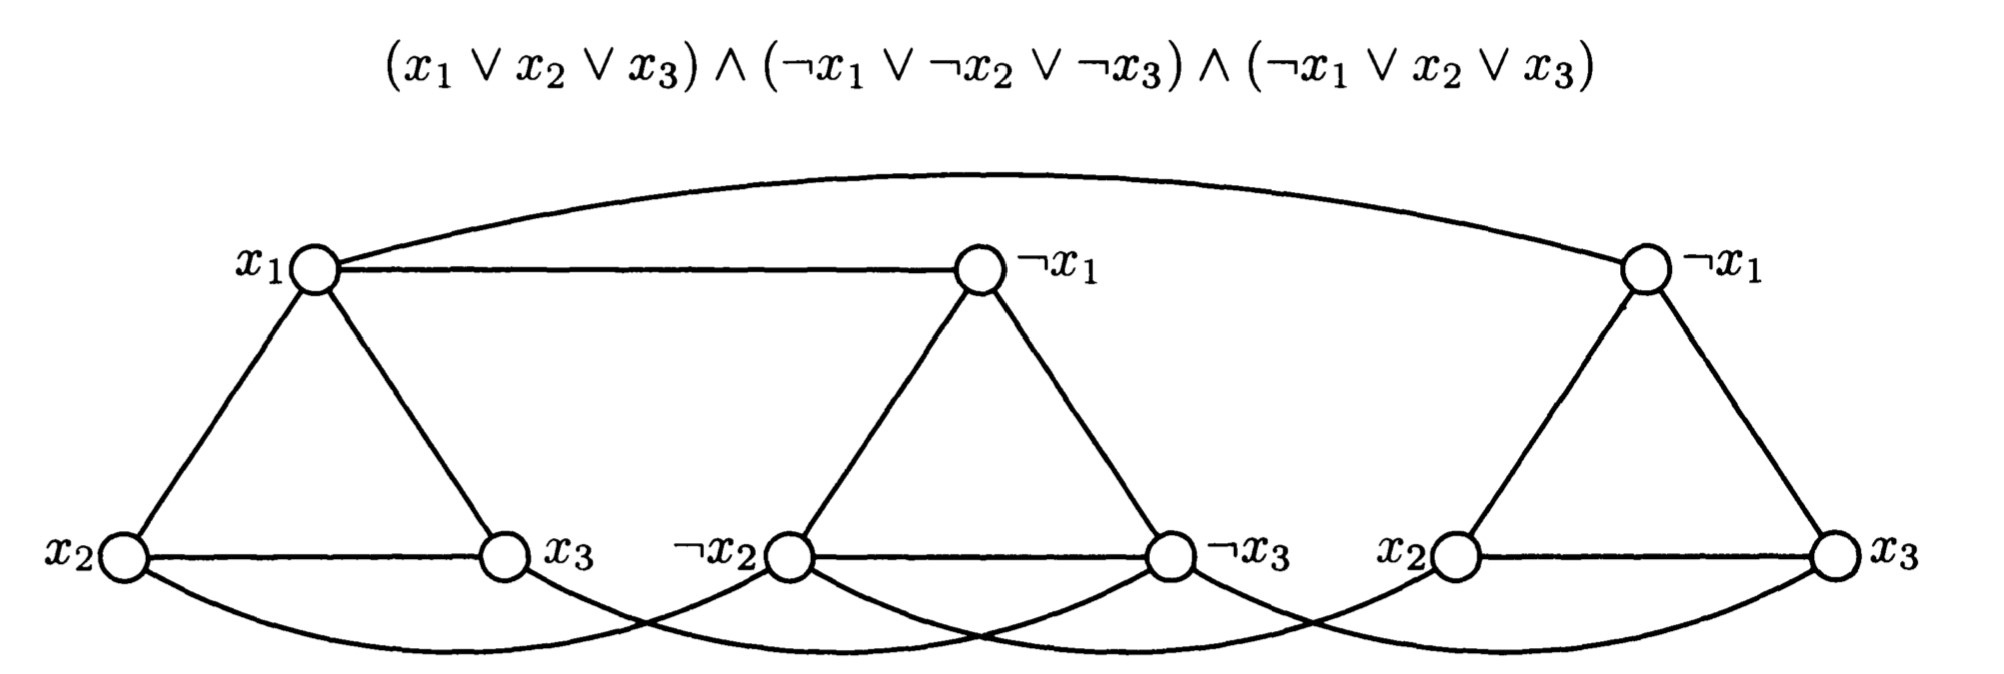
\includegraphics[scale=0.5]{triangle.jpg}
\end{center}
\caption{Graph with triangles \cite{book}}
\end{figure}
\item consider only graphs whose nodes can be partitioned in $m$ disjoint triangles \\
$\rightarrow$ independent set can contain at moast $m$ nodes (one from each triangle)
\item reduction from \textsc{3Sat} to \textsc{IndependentSet}
\item construct graph of formula $\phi$:
\begin{itemize}
\item each literal as a node
\item clauses as triangles
\item edges between nodes in different triangles if they correspond to the same literal (negated)
\item $K = m$ ($m$ clauses) 
\end{itemize}

\item given: instance $\phi$ of \textsc{3Sat} with $m$ clauses $C_1,...,C_m$
\item each clause $C_i=(\alpha_{i1} \lor \alpha_{i2} \lor \alpha_{i3})$ (with $\alpha$ as boolean variables or negation of those)
\item reduction $R$ constructs a graph: $R(\phi) = (G, K)$ where $K=m$ and $G=(V,E)$
\item nodes $V = \{ v_{ij}: \ i = 1, ..., m; j = 1, 2, 3 \}$ \\
nodes for each of the $m$ clauses ($i$) for each of the 3 literals ($j$)
\item edges $E = \{ [ v_{ij}, v_{ik}  ] : \ i = 1, ..., m; j \neq k \} \cup \{ [ v_{ij}, v_{lk}  ] : \ i  \neq l, \alpha{ij} = \neg \alpha_{lk} \}$ \\
edges between the nodes in one clause (triangle edges) \\
edges between nodes with the same corresponding literal, but negated\\

\item there is an indepentent set $I$ of $K$ nodes in $G$ only if $\phi$ is satisfiable
\item $I$ must contain a node from each triangle
\item negated literals are connected: $I$ cannot contain a literal and its negation
\item $I$ is a truth assignment of $\phi$:
\begin{itemize}
\item true literals: nodes in $I$
\item one true literal per clause
\end{itemize}

\end{itemize}





%---------------------------------------------------------------








\subsection*{\textsc{HamiltonPath} is NP-complete}


\begin{CountingDefinition}[\textsc{HamiltonPath}]{def:validLabelPlacement}
A \textsc{HamiltonPath} is a path in a graph that visits each node exactly once.
\end{CountingDefinition}

\textsc{HamiltonPath} is NP-complete.

\ \\
\textbf{Proof idea:}
\begin{itemize}
\item reduction from \textsc{3Sat} to \textsc{HamiltonPath}
\item given: formula $\phi$ in CNF with $n$ variales $x_1,...,x_n$ and $m$ clauses $C_1,...,C_m$ with each 3 variables
\item construct a graph $R(\phi)$ that has a hamilton path only if $\phi$ is satisfiable:

\item boolean variables:

\begin{itemize}
\item choice between true and false
\item all occurences of $x$ must have the same value (and $\neg x$ the opposite)
\item use \textit{choice} gadget (like flip flop)
\end{itemize}

\item XOR:

\begin{itemize}
\item[]
\begin{figure}[H]
\begin{center}
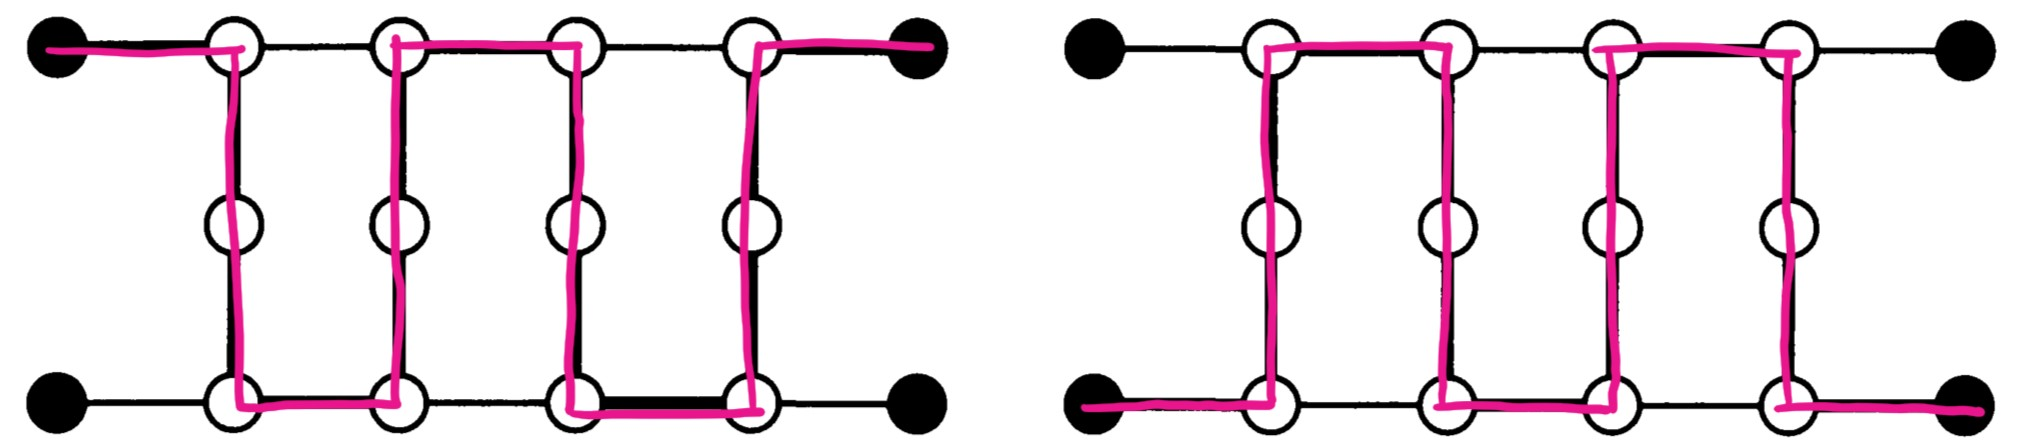
\includegraphics[scale=0.5]{xor.jpg}
\end{center}
\caption{XOR subgraph from the book \cite{book} with the relevant edges marked additionally}
\end{figure}
\item use \textit{consistency} gadget
\item because of hamilton path: there are only two ways to traverse through this sub graph (as shown above)
\item leads to exclusive or (XOR)
\item[]
\begin{figure}[H]
\begin{center}
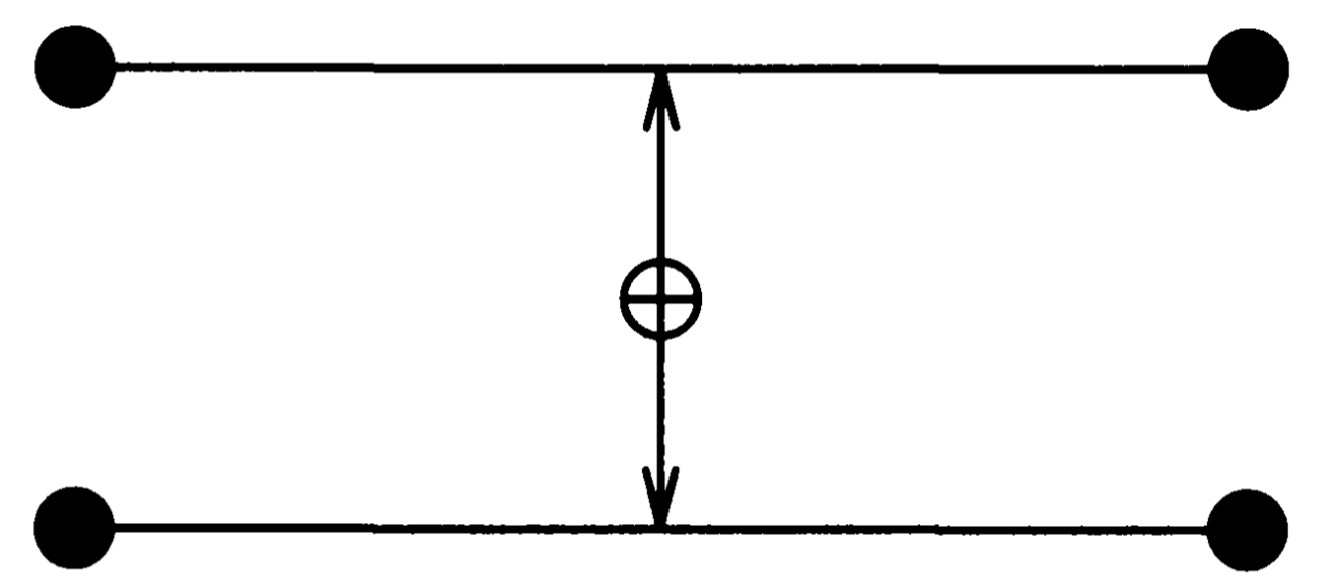
\includegraphics[scale=0.3]{xor2.jpg}
\end{center}
\caption{XOR connecting two independent edges (\textit{consistency} gadget) \cite{book}}
\end{figure}
\end{itemize}

\item clauses:
\begin{itemize}
\item triangles for clause construction
\item one side for each literal
\item if literal is false: hamilton path traveres triangle side
\item at least one literal need to be true: else all three edges of triangle will be traversed and this is not a hamilton path 
\end{itemize}

\item put everything together as graph $G$:
\begin{itemize}
\item $G$ has $n$ copies of the \textit{choice} gadget as a chain (one for each variable)
\item[]
\begin{figure}[H]
\begin{center}
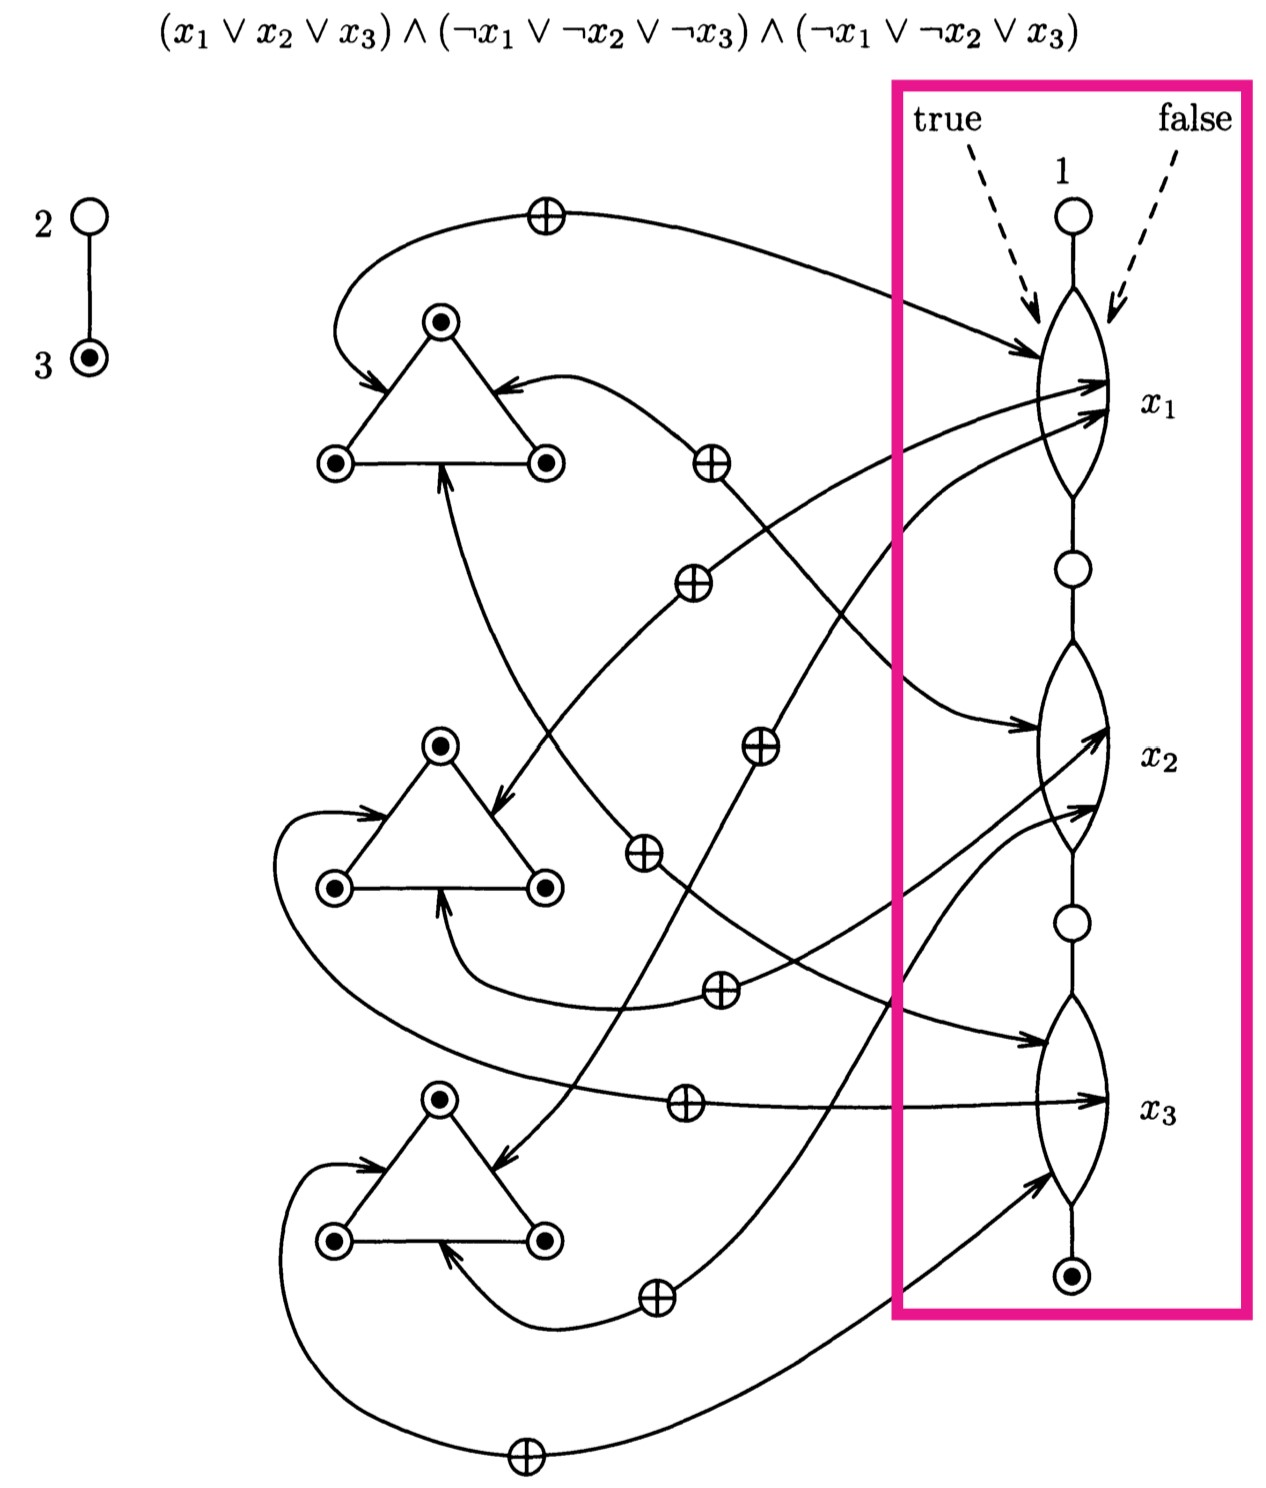
\includegraphics[scale=0.4]{choicegadgets.jpg}
\end{center}
\caption{\textit{Choice} gadgets marked in graph from the book \cite{book}}
\end{figure}
\end{itemize}

\item $G$ has $m$ triangles (one for each clause) with edges for each clause in the triangle
\begin{itemize}
\item[]
\begin{figure}[H]
\begin{center}
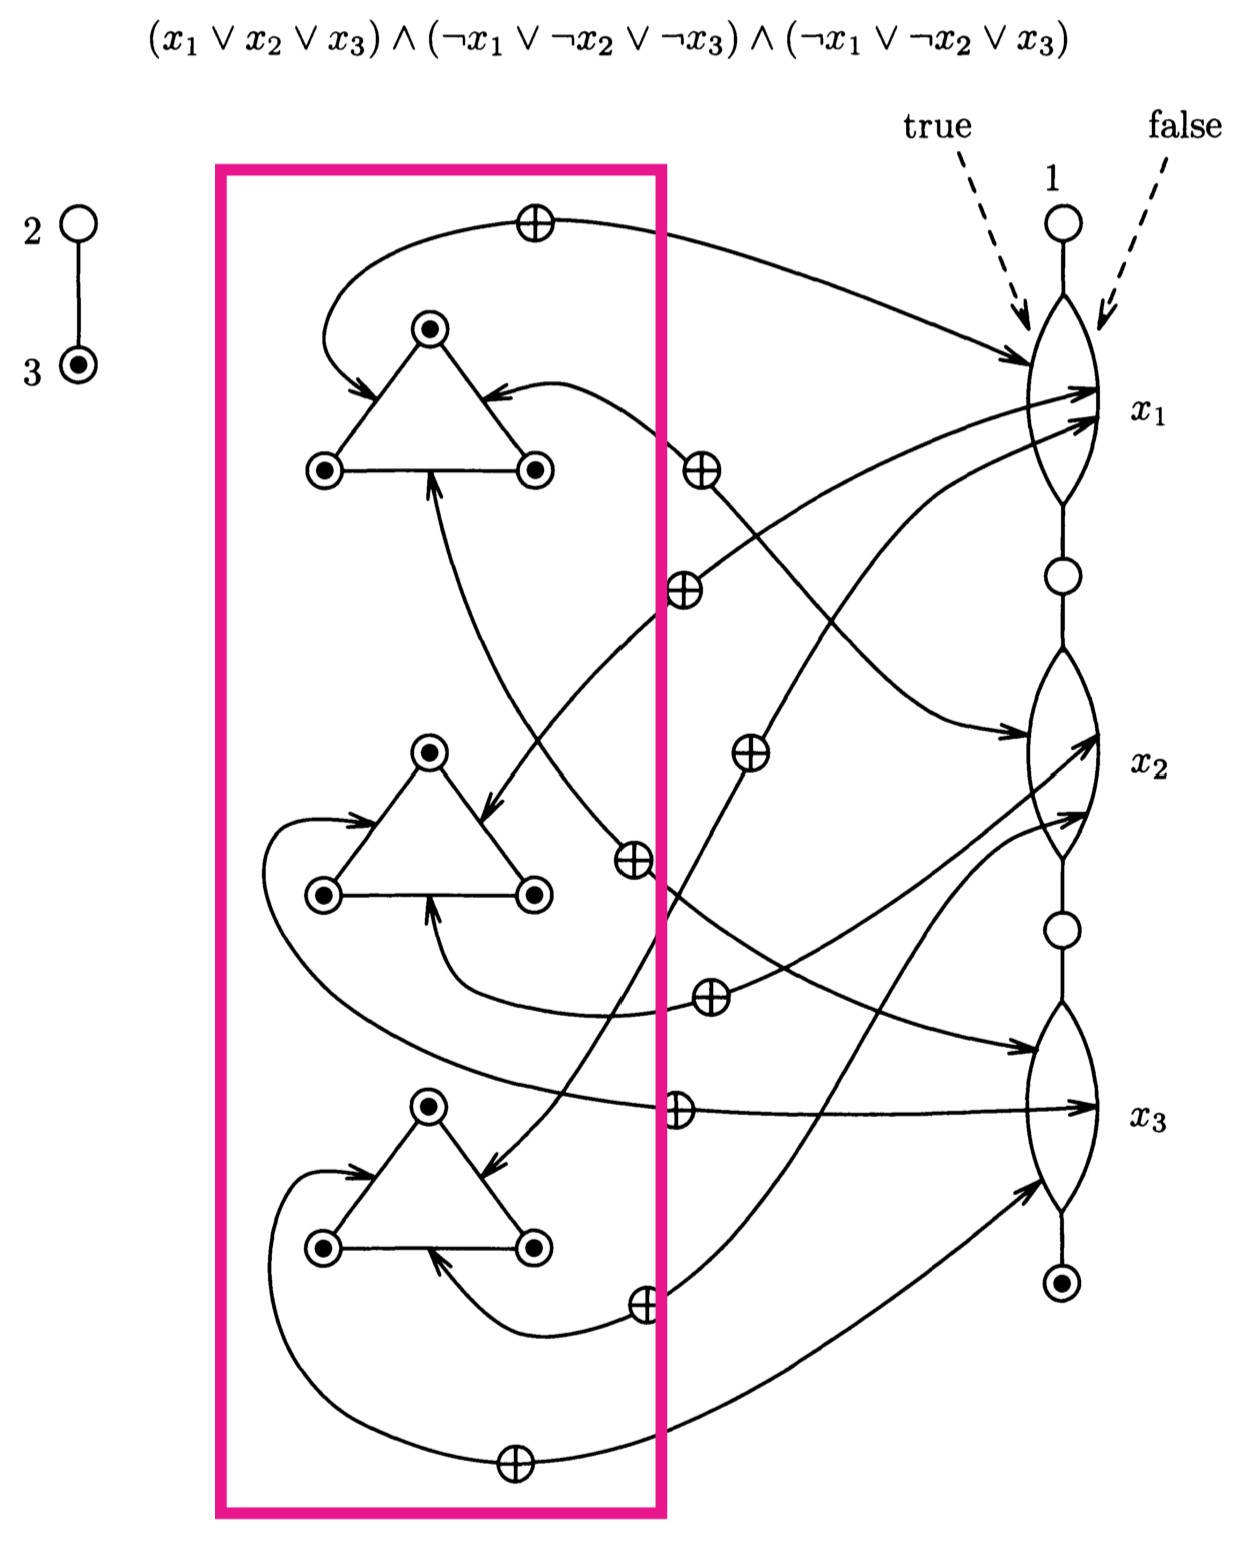
\includegraphics[scale=0.4]{triangle2.jpg}
\end{center}
\caption{Clauses marked in graph from the book \cite{book}}
\end{figure}
\end{itemize}

\item finally all $3m$ nodes of the triangles, the last node of the chain of \textit{choice} gadgets and a new node 3 are connected with all possible edges
\item a single node 2 is connectes to the node 3 \\
\begin{itemize}
\item[]
\begin{figure}[H]
\begin{center}
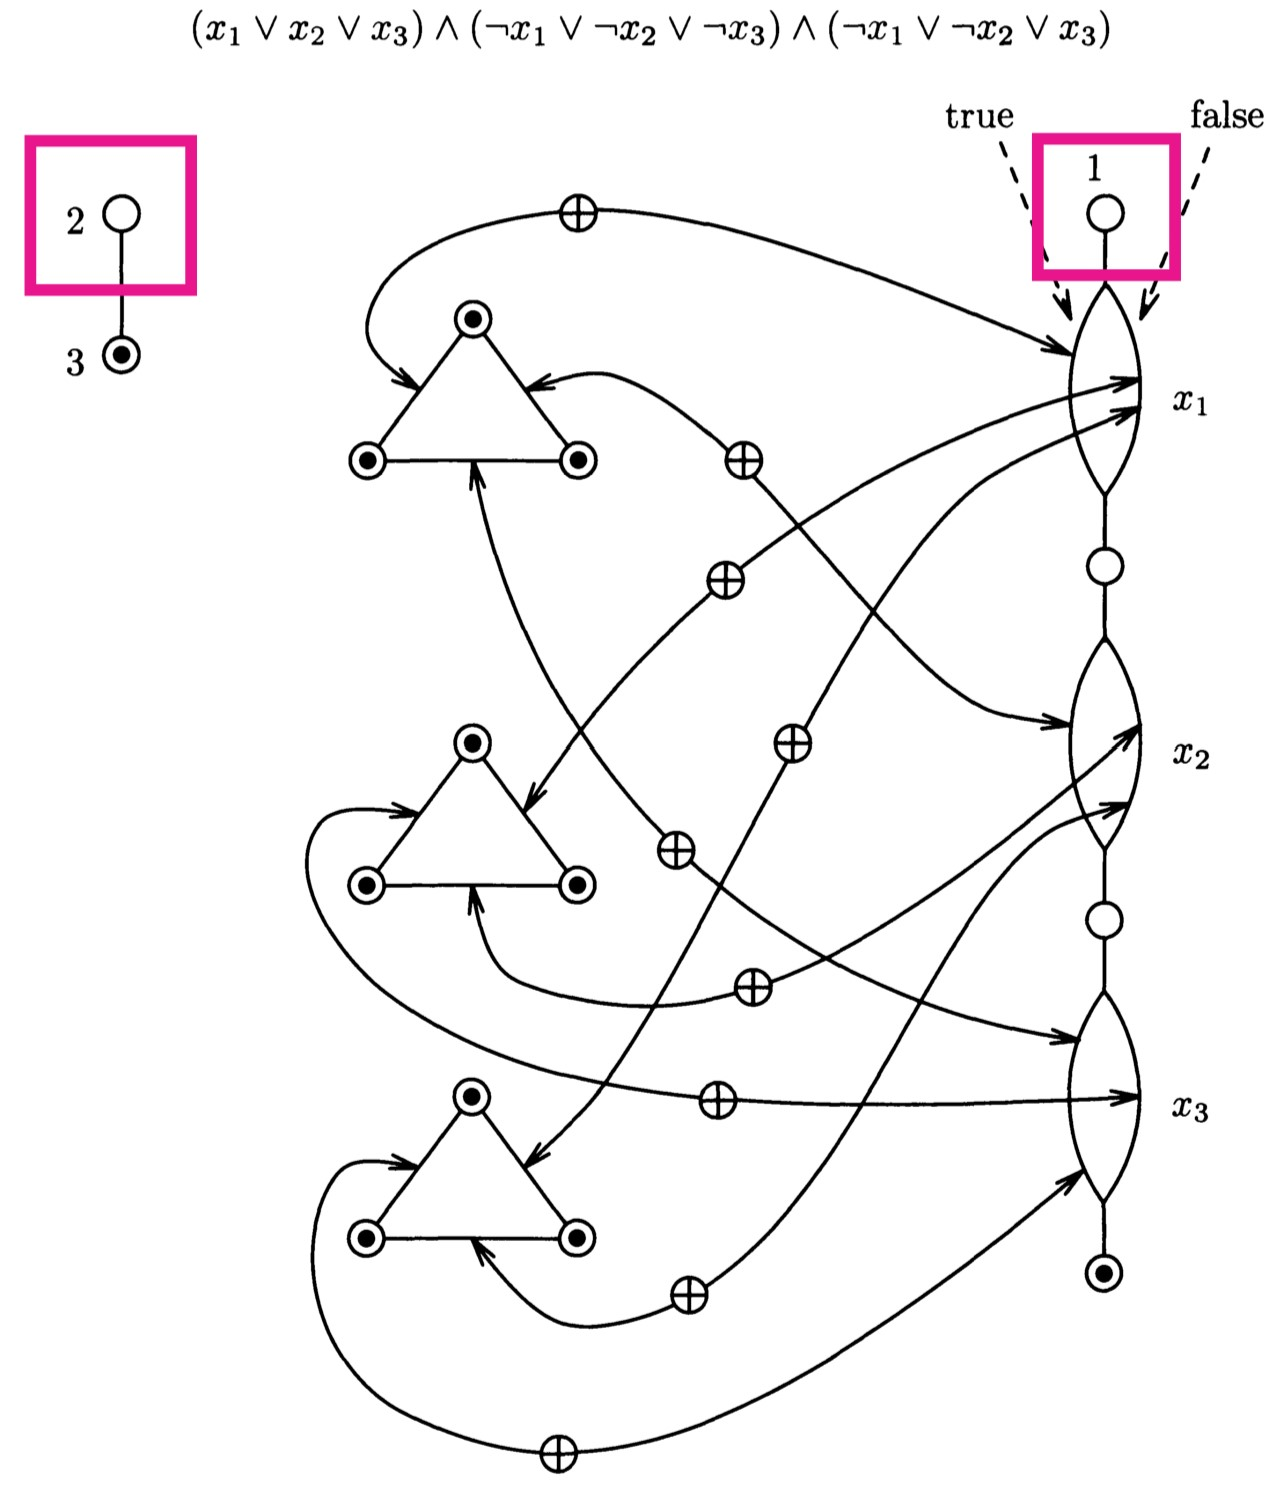
\includegraphics[scale=0.4]{12.jpg}
\end{center}
\caption{Nodes 1 and 2 marked (start and end node) in graph from the book \cite{book}}
\end{figure}
\end{itemize}

\item graph has a hamilton path only if $\phi$ has a satisfying truth assignment
\item for hamilton path: start node is node 1 and end node is node 2
\item from node 1 it must traverse one of the parallel edges of the \textit{choice} gadget for the first variable
\item exclusive ors must be traversed
\item whole chain of \textit{choice} gadgets will be traversed \\
$\rightarrow$ in this way a truth assignment $T$ is created
\item then the triangles are traversed and it ends up in node 2 if there is a hamilton path and $\phi$ is satisfyable


\end{itemize}




%---------------------------------------------------------------











\subsection*{\textsc{TSP(D)}}

\begin{CountingDefinition}[\textsc{TSP(D)}]{def:validLabelPlacement}

\textsc{TSP(D)} is a decision version of \textsc{TSP}.
\ \\
Input: A $n \times n$ distance matrix and a bound $B \in \mathbb{N}$
\ \\
Question: Is there a round tour of length $\leq B$ that visits all \textit{cities}?
\end{CountingDefinition}

\textsc{TSP(D)} is NP-complete.

\ \\
\textbf{Proof idea:}
\begin{itemize}
\item reduce from \textsc{HamiltonPath} to \textsc{Tsp}
\item given: graph $G$ with $n$ nodes
\item design: matrix $d_{ij}$ and a budget $B$ of nodes with $B = |V| + 1$ such that there is a tour of length $B$ or less only if the $G$ has a hamilton path
\item $d_{ij}$ usually contains the distance from city $i$ to city $j$
\item $n$ cities: one node for each city in the graph \\
$\rightarrow$ $n$ nodes
\item distance between two cities $i$ and $j$ is 1 if there is an edge $[i,j]$ and 2 otherwise
\end{itemize}


\textbf{Example:} \ \\


%------------------------------------

\begin{minipage}{0.7\textwidth}
\begin{figure}[H]
\begin{center}
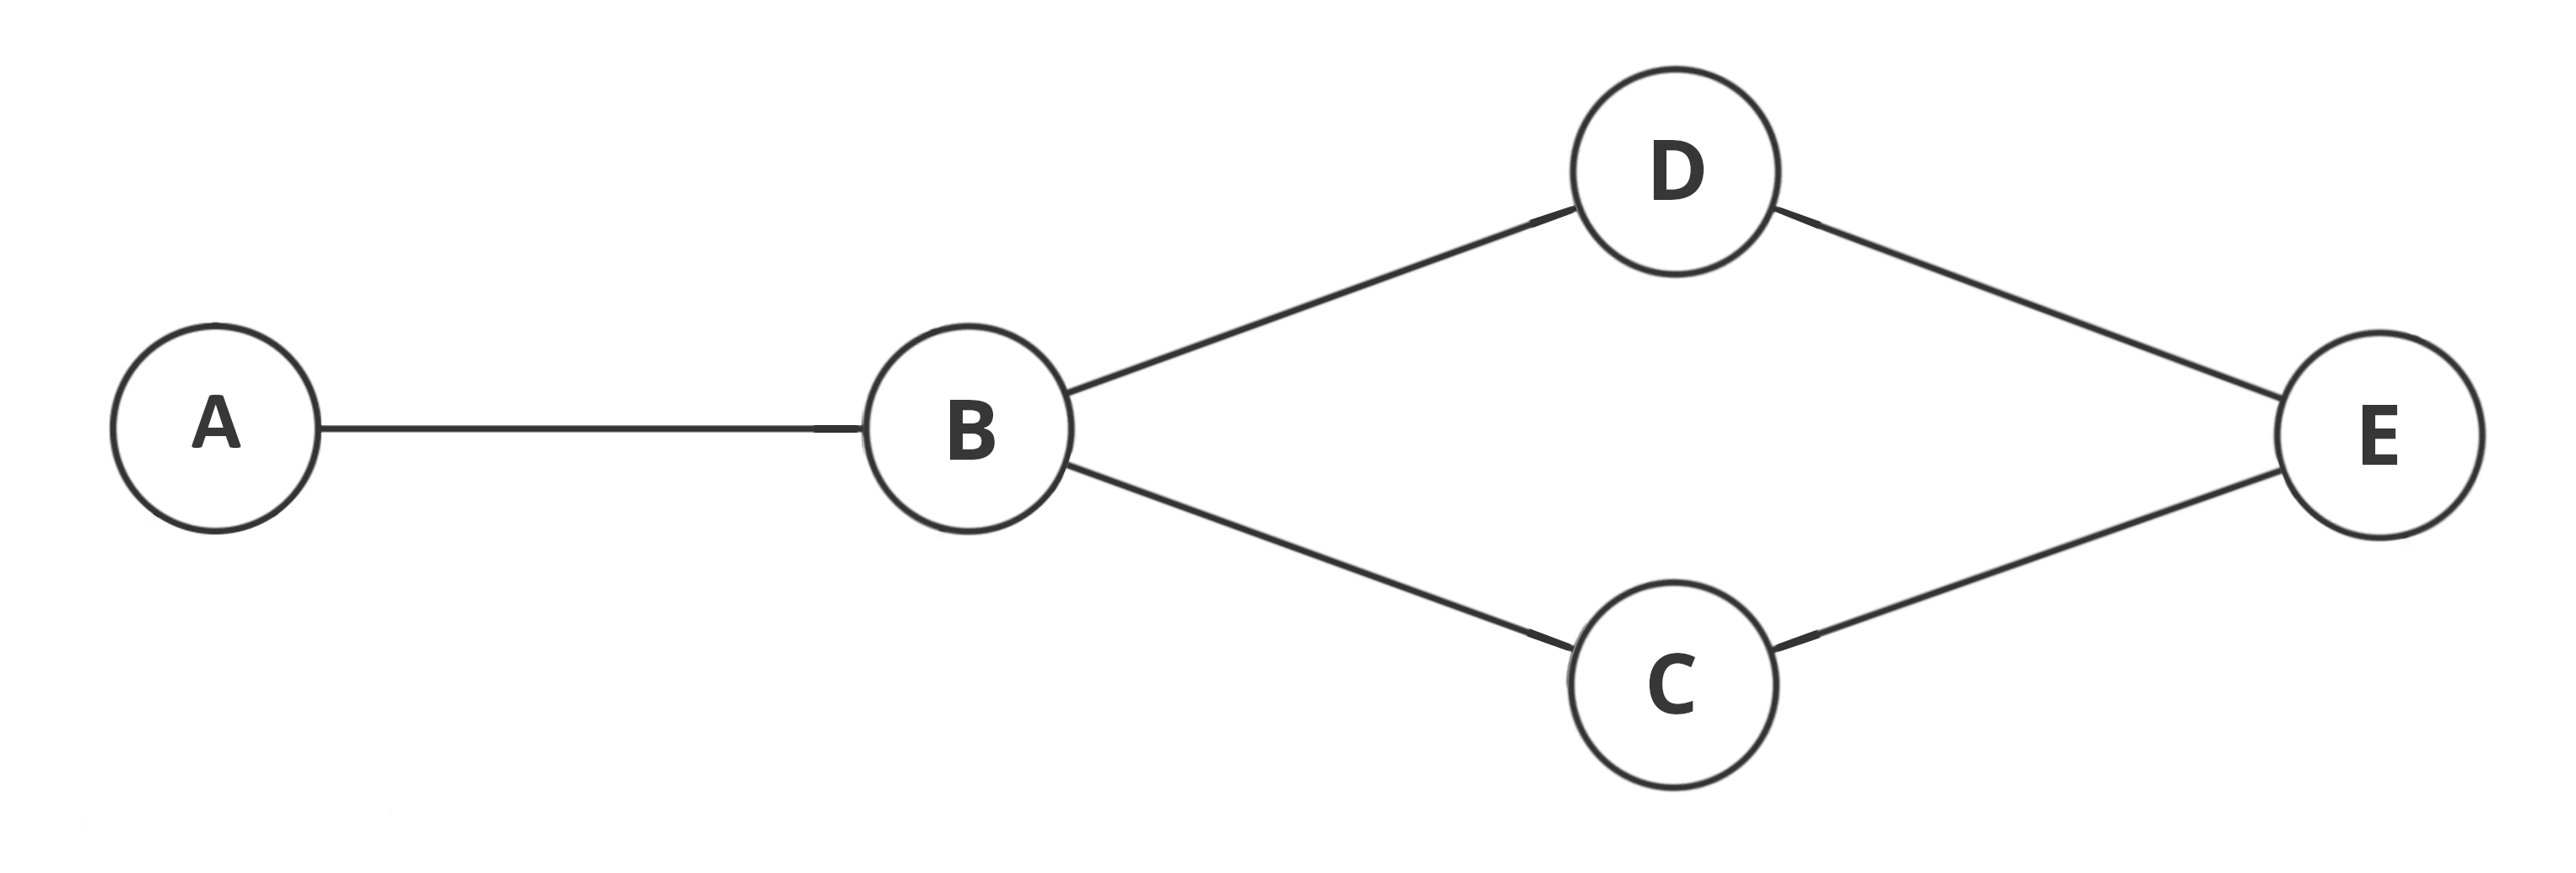
\includegraphics[scale=0.18]{tsp_1.png}
% \includegraphics[scale=0.4]{tsp3.jpg}
\end{center}
\caption{Corresponding table to the graph}
\end{figure}

\end{minipage}\begin{minipage}{0.05\textwidth}
\ \\
\end{minipage}\begin{minipage}{0.25\textwidth}
\begin{tabular}{c|c|c|c|c|c|}
 & A & B & C & D & E \\
\hline
A & -- & 1 & 2 & 2 & 2 \\
\hline
B & 1 & -- & 1 & 1 & 2 \\
\hline
C & 2 & 1 & -- & 2 & 1 \\
\hline
D & 2 & 1 & 2 & -- & 1 \\
\hline
E & 2 & 2 & 1 & 1 & -- \\
\hline
\end{tabular}


\end{minipage}

\begin{itemize}
\item undirected: distances are symmetric, leads to $d_{ij} = d_{ji}$
\item set limit to $B = |V|+1 = 6$
\item $\sum^{n}_{i=1} d_{\pi(i), \pi(i+1)}$ is as small as possible
\item $\pi$ is a permutation
\item[] The following sum for the example can at most be 6:
\begin{align*}
 \text{A to B: } & \  d_{\pi(0), \pi(1)} =  1 \\
  \text{B to C: } & \  d_{\pi(1), \pi(2)} = 1\\
   \text{C to E: } & \  d_{\pi(2), \pi(3)} = 1 \\
 \text{E to D: } & \  d_{\pi(3), \pi(4)} =  1\\
 \text{D to A: } & \  d_{\pi(4), \pi(0)} = 2
 \\
 & \ \sum = 6
\end{align*}
\item the answer to the \textsc{Tsp} problem is \textit{yes}
\item the graph contains a hamilton path
\end{itemize}





%------------------------------------

%\begin{minipage}{0.7\textwidth}
%\begin{figure}[H]
%\begin{center}
% \includegraphics[scale=0.18]{tsp_2.png}
% \includegraphics[scale=0.4]{tsp3.jpg}
%\end{center}
%\caption{Corresponding table to the graph}
%\end{figure}

%\end{minipage}\begin{minipage}{0.05\textwidth}
%\ \\
%\end{minipage}\begin{minipage}{0.25\textwidth}
%\begin{tabular}{c|c|c|c|c|c|}
% & A & B & C & D & E \\
%\hline
%A & -- & 1 & 2 & 2 & 2 \\
%\hline
%B & 1 & -- & 1 & 2 & 2 \\
%\hline
%C & 2 & 1 & -- & 2 & 1 \\
%\hline
%D & 1 & 2 & 2 & -- & 1 \\
%\hline
%E & 2 & 2 & 1 & 1 & -- \\
%\hline
%\end{tabular}


%\end{minipage}

%\begin{itemize}
%\item undirected: distances are symmetric, leads to $d_{ij} = d_{ji}$
%\item set limit to $B = |V|+1 = 6$
%\item $\sum^{n}_{i=1} d_{\pi(i), \pi(i+1)}$ is as small as possible
%\item $\pi$ is a permutation
%\item[] The following sum for the example can at most be 6:
%\begin{align*}
% \text{A to B: } & \  d_{\pi(0), \pi(1)} =  1 \\
%  \text{B to C: } & \  d_{\pi(1), \pi(2)} = 1\\
%   \text{C to E: } & \  d_{\pi(2), \pi(3)} = 1 \\
% \text{E to D: } & \  d_{\pi(3), \pi(4)} =  1\\
% \text{D to A: } & \  d_{\pi(4), \pi(0)} = 1
% \\
% & \ \sum = 5
%\end{align*}
%Answer to \textsc{Tsp} is \textit{yes}.
%\end{itemize}


\ \\
\color{red} TODO \\
proof \\
\color{black}
\color{violet} Questions:
\color{black}

%---------------------------------------------------------------












\subsection*{\textsc{Knapsack}}



\begin{CountingDefinition}[\textsc{Knapsack}]{def:validLabelPlacement}
Given is a set of items with a weight and a value. The task is to choose which items to include so that the total weight is less than the given limit of the knapsack and the total value is as large as possible.
\end{CountingDefinition}

Recalling my Dynamic Programming knowledge for the \textsc{Knapsack} problem \\
The formula for the dynamic programming of this problem is the following:

  $$
Opt(i,j)=
\begin{cases}
0, & \text{for } 0\leq j \leq size\\
        Opt(i-1, j), & \text{for } j < w[i]\\
        max\{ Opt(i-1, j), v[i]+Opt(i-1, j-w[i]) \}, & \text{else } 
\end{cases}
$$

\begin{itemize}
\item if $0 \leq j \leq w$: there are no objects which could be put into the bag
\item second case: object $i$ does not fit into the bag and the optimal solution is found with the objects from index $1$ to $i-1$
\item else: object $i$ is either part of the optimal solution or it consists out of the objects $1$ to $i-1$
\end{itemize}

Table fill-out example:
\begin{itemize}
\item left: table of the values and weight of each item with index $i$ is shown on the left 
\item right: table that gets filled in with a dynamic programming approach of the formula above, the maximum bag size is 7
\item first column in the table represent the objects and the last row the weight 
\item entries in the table show the maximum value
\item maximum value for the size 7 is 10.
\end{itemize}
\begin{minipage}{0.3\textwidth}

\begin{tabular}{|c|c|c|}
\hline
$i$ & $w[i]$ & $v[i]$ \\
\hline
1 & 1 & 1 \\
2 & 3 & 4 \\
3 & 2 & 3 \\
4 & 4 & 6 \\
5 & 6 & 8 \\
\hline
\end{tabular}


\end{minipage}\begin{minipage}{0.1\textwidth}
\ 
\end{minipage}\begin{minipage}{0.6\textwidth}

\begin{tabular}{|c||c|c|c|c|c|c|c|c|}
\hline
5 & 0 & 1 & 3 & 4 & 6 & 7 & 9 & 10 \\
\hline
4 & 0 & 1 & 3 & 4 & 6 & 7 & 9 & 10 \\
\hline
3 & 0 & 1 & 3 & 4 & 5 & 7 & 8 & 8 \\
\hline
2 & 0 & 1 & 1 & 4 & 5 & 5 & 5 & 5 \\
\hline
1 & 0 & 1 & 1 & 1 & 1 & 1 & 1 & 1 \\
\hline
0 & 0 & 0 & 0 & 0 & 0 & 0 & 0 & 0 \\
\hline
\hline
  & 0 & 1 & 2 & 3 & 4 & 5 & 6 & 7 \\
\hline

\end{tabular}

\end{minipage}

\ \\

\begin{CountingDefinition}[\textsc{ExactCoverBy3Sets}]{def:validLabelPlacement}
Given a set $X$, with $|X| = 3q$ (so, the size of $X$ is a multiple of $3$), and a collection $C$ of 3-element subsets of $X$.  Can we find a subset $C'$ of $C$ where every element of $X$ occurs in exactly one member of $C'$?  (So, $C'$ is an exact cover of $X$).
\end{CountingDefinition}


\textsc{Knapsack} is NP-complete.

\ \\
\textbf{Proof idea:}
\begin{itemize}
\item special case of \textsc{Knapsack} where $v_i = w_i$ and $K = W$
\item $K$ is the goal value (sum of values $v_i$ needs to be greater than $K$)
\item $W$ is the maximum bag size (sum of weights $w_i$ has to be smaller than $W$)
\item given: set of $n$ integers $w_i,...,w_n$ and an integer $K$
\item find: subset of the given integers that sums up exactly to $K$ \\

\item

\end{itemize}













\color{red} TODO \\
\color{black}
\color{violet} Questions:
\color{black}

%---------------------------------------------------------------


\newpage

\printbibliography




\end{document}
